\documentclass[10pt,draftclsnofoot,onecolumn,compsoc]{IEEEtran}
\usepackage[letterpaper, portrait, margin=0.75in]{geometry}
%\usepackage[myheadings]{fullpage}
\usepackage{fancyhdr}
\usepackage{lastpage}
\usepackage{graphicx,  subcaption,  booktabs}
\usepackage[T1]{fontenc}
\usepackage[font=small, labelfont=bf]{caption}
%\usepackage{fourier}
\usepackage[protrusion=true, expansion=true]{microtype}
\usepackage[english]{babel}
%\usepackage{sectsty}
\usepackage{url, lipsum}
\usepackage{tikz}
\usepackage[section]{placeins}
%\usepackage{makeidx}
\newcommand{\subparagraph}{}
\usepackage{titlesec}
\usepackage{enumitem}

\makeatletter
\renewcommand{\@IEEEsectpunct}{ \\ \\ \,}% Modified from {:\ \,}
\makeatother

\setlength{\parindent}{0em}
\setlength{\parskip}{1em}
\renewcommand\thesection{\arabic{section}}
\renewcommand\thesubsection{\thesection.\arabic{subsection}}
\renewcommand\thesubsubsection{\thesubsection.\arabic{subsubsection}}

\makeatletter
\renewcommand\paragraph{\@startsection{paragraph}{4}{\z@}%
                                    {0ex \@plus0ex \@minus.0ex}%
                                    {0em}%
                                    {\normalfont\normalsize\bfseries}}
\makeatother

\renewcommand\thesectiondis{\arabic{section}}
\renewcommand\thesubsectiondis{\thesectiondis.\arabic{subsection}}
\renewcommand\thesubsubsectiondis{\thesubsectiondis.\arabic{subsubsection}}


\titleformat{\section}
       {\normalfont\fontfamily{phv}\fontsize{14}{17}\bfseries}{\thesection}{1em}{}
\titleformat{\subsection}
       {\normalfont\fontfamily{phv}\fontsize{14}{17}\bfseries}{\thesubsection}{1em}{}
\titleformat{\subsubsection}
       {\normalfont\fontfamily{phv}\fontsize{14}{17}\bfseries}{\thesubsubsection}{1em}{}


\newcommand{\namesigdatehrule}[1]{\par\tikz \draw [blue, densely dotted, ultra thick] (0,0) -- (#1,0);\par}
\newcommand{\namesigdate}[2][5cm]{%
\begin{minipage}{#1}%
    #2 \vspace{0.8cm}\namesigdatehrule{#1}\smallskip
    \small \noindent\textit{Signature}
    \vspace{0.8cm}\namesigdatehrule{#1}\smallskip
    \small \textit{Date}
\end{minipage}
}


\newcommand{\HRule}[1]{\rule{\linewidth}{#1}}
\newcommand*\tick{\textsc{\char13}}
\linespread{1}
\setcounter{tocdepth}{5}
\setcounter{secnumdepth}{5}

\makeindex

\begin{document}
%\title{HyRo}
%\author{Jason Klindtworth  |  Josh Asher  |   Layne Nolli}
%\date{}
%\maketitle
\begin{titlepage}
	\centering
	{\scshape\LARGE HyRo \par}
	%\vspace{1cm}
	{\scshape\LARGE Team 28\par}
	\vspace{1cm}
	{\scshape\Large Jason Klindtworth  |  Josh Asher  |   Layne Nolli}
	\noindent\makebox[\linewidth]{\rule{17cm}{2pt}}
	\vspace{1cm}
	{\huge\bfseries CS463\par}
	\vspace{2cm}
	{\Large\itshape Spring 2017\par}
	\vspace{4cm}
	{\large Software Design Document\par}\vspace{2cm}
	{\large Abstract\par}
	\vspace{1cm}
	High Altitude rockets have a distinct advantage in using Hybrid propulsion systems. These systems are complex and present challenges in remote telemetry including launch initialization and controlling remote fuel filling/disconnect. High altitude rockets contain an array of sensors that collect data which needs to be represented in human-readable format. The goal of HyRo is to provide solutions for remotely launching and controlling the fuel systems on a hybrid propulsion system through onboard embedded circuitry/software that communicates with the launch team via radio waves. Our solutions will make use of a python-based GUI for ground teams to interface with. Sensor data is displayed on our graphical user interface in an appealing, human-readable way. \par

	\noindent\makebox[\linewidth]{\rule{17cm}{2pt}}
	\vfill

% Bottom of the page
	{\large \today\par}
\end{titlepage}


\setcounter{tocdepth}{2}
\tableofcontents
\newpage

\section{Introduction}
\subsection{Scope}
This Design Document describes in detail, both the structure, and components of the HyRo deployment software system. It also includes the implementation details required to accurately and completely incorporate the specific requirements of this project as described in the Requirements Document. Because of the nature of the content in this document, it is assumed that the reader has familiarized themselves with the projects Requirements Document and is aware of the specific needs of this software package and graphical user interface. There is also an assumed general knowledge of computer programing. This document will rely heavily on the explanation of specific software functions and processes that will be designed in order to satisfy all of the requirements for this project. 
\subsection{Purpose}
This Design Document serves the following purposes:
\begin{itemize}
	\item To fully describe the structure, functions, data, and algorithms to be implemented in the software package.
	\item To identify specific and general system resources that will be utilized.
	\item To assist the HyRo team in the production and implementation of test cases.
	\item To verify full compliance with the requirements of the project.
	\item To aid the team in the general overview of the software package and what its capabilities are.
\end{itemize}
\subsection{Intended Audience}
The majority of the document is written for the benefit of software development and design professionals in order to gain specific knowledge of the HyRo software system and its capabilities. The intended audience for this documents is the HyRo team, including the following:
\begin{itemize}
	\item The project supervisor 
	\item The computer science sub-team working on the software package itself.
	\item The electrical engineering sub-team working on the hardware the software package will be incorporated into.
	\item The mechanical engineering sub-team working on the mechanical operations of the rocket which the software/hardware package will ride on.
	\item Any related sub-team for the project that requires knowledge of the computer system or interface system for the rocket.
\end{itemize}
\subsection{Definitions}
\begin{description}
	\item[Hybrid Rocket] A rocket with an engine that uses both solid and liquid fuel.
	\item[I/O] Input and Output.
	\item[PWM] Pulse Width Modulation is used to control signal level on a electrical wire.
	\item[Beagle Bone Black] A miniature computer that will be used on-board our hybrid rocket to house our software.
	\item[Python Dictionary] A associative array accessed by key value pairs.
	\item[Oxidizer] Liquid gas used to accelerate the burning of solid fuel.
	\item[Accelerometer] Measures acceleration.
	\item[Gyroscope] Measure tilt relative to the earth.
	\item[Magnetometer] Measures the electric field around it.
	\item[Multi Threaded] A program that runs multiple methods in parallel to the main program allowing components to run independently.
	\item[Mutex Lock] Used to lock control of an area of memory while an operation is completed. If any other parts of the system attempt to access this part of memory while the lock is in place they will not be allowed to.
	\item[Boolean] A way to represent a true or false value in software.
\end{description}
\subsection{Overview}
The HyRo software system is composed of two major components. The first component is housed on-board a hybrid rocket. This component is responsible for gathering sensor data from sensors on the the rocket, sending this data to a ground computer, and receiving commands from the ground system. These commands will interact with electrical components on the rocket. This component will be developed by the ECE sub steam and its design is not part of this document. The second component of this system is software running on a traditional computer that is located on the ground near the launch site. This is the component we are responsible for. Our software is responsible for presenting the user with a graphical user interface that will allow the sending of commands to the rocket. It will also monitor data from the rocket that will be represented in graphs and gauges. The graphical user interface backend will also log any important information or commands that the rocket team requests. The main purpose of our project is to provide remote filling, data visualization, and data logging. This paper is sectioned into 2 views. The first view System Architecture on the traditional computer, is explained from a logical viewpoint. The final section, the user interface, is explained from an interface viewpoint.
\section{Stake Holders and Concerns}
The primary stake holders in this project are Nancy Squires and the hybrid rocket team collectively. The rocket team is composed of Mechanical Engineering students, Electrical Engineering Students, and Computer Science Engineering students. We all have the same design concerns. These concerns include remotely filling and visualizing data from a rocket. The most important thing is to be able to visualize sensor data while the rocket is in flight and again after the data has been collected and stored. This communication needs to be fast and accurate. This project is an ongoing process and its design will be a living entity. Things will change and we must adapt our design to these changes as the project progresses.

\begin{figure}[!ht]
  \caption{Data Flow Between System Components.}
  \centering
	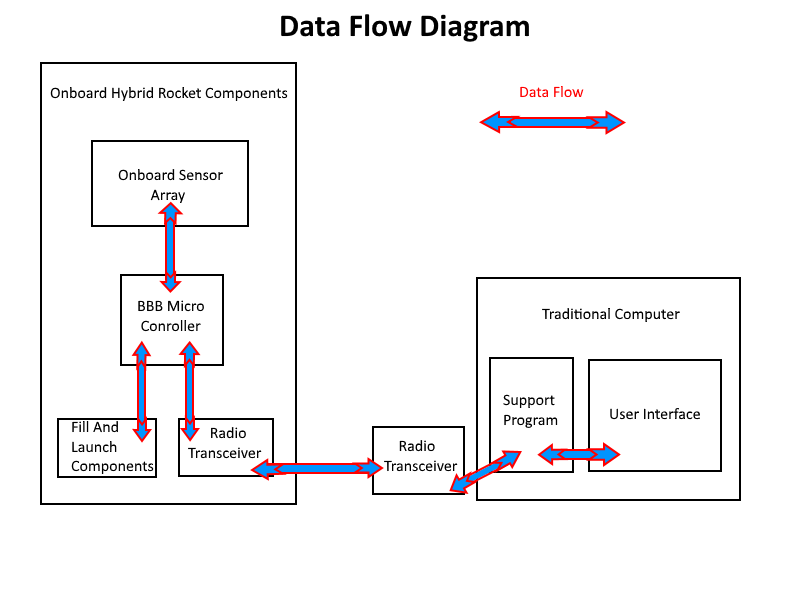
\includegraphics[scale=.85]{RocketBlockDiagram}
\end{figure}
\FloatBarrier


\section{System Architecture on a Traditional Computer }
The SDD module design of the software running on a traditional computer detailed here after will explain the approach, methods, and properties of this component of the system. Software running on the traditional computer will communicate to the ECE subsystem onboard the rocket. This component of the system will be responsible for monitoring radio transmissions, sending commands, logging, replaying logged data, and the user interface back end. \par

\subsection{Overview}
In the following sections we describe the components of this software, excluding the user interface which is described in depth in the next section. We go over the graphical back end toolkits that will be used to draw the user interface, the data format of queues( buffers) and logs, worker threads, button listener functions, data conversion functions, and data visualization functions (drawing functions). \par

\subsection{GUI and Graphing Toolkits}
We will be using the Python TKinter library which provides a basis for windows, buttons, canvas, and other varies components we will need to create our graphical interface. This library includes event listeners to easily detect button presses and a canvas to easily draw gauges and graphs. All sub components like buttons are called widgets in TKinter. \par
On top of Tkinter we will be using Matplotlib which is a graphical plotting library. Matplotlib provides functions to be easily able to graph data and scale those graphs. Graphs will be drawn on TKinter canvas widgets. To provide numerical integration of velocity we are using the Scipy library.\par

\subsection{Data Format}

\begin{description}
	\item[Data Buffers] Queues that hold sensor information before processing.
	\item[Queue Names]  -
	\begin{description}
		\item[altitude] The altitude above ground level reading from the altitude sensor.
		\item[temp] The temperature reading from the temperature sensor.
		\item[a\_x] Accelerometer data from x axis.
		\item[a\_y] Accelerometer data from y axis.
		\item[a\_z] Accelerometer data from z axis.
		\item[g\_x] Gyroscope data from the x axis.
		\item[g\_y] Gyroscope data from the y axis.
		\item[g\_z] Gyroscope data from the z axis.
		\item[m\_x] Magnetometer data from the x axis.
		\item[m\_y] Magnetometer data from the x axis.
		\item[m\_z] Magnetometer data from the x axis.
		\item[tank\_pres] The pressure of the oxidizer tank. **This is a stretch goal at the moment.
		\item[chamber\_pres] The pressure of the combustion chamber. **This is a stretch goal at the moment.
	\end{description}
\end{description}

\subsubsection{Sensor Data Buffer}
The sensor data buffer will be individual queues each relating to a sensor component on board the rocket. As data is received by the XBee it will be placed on these Queues to be operated on by the main thread.
\begin{description}
	\item[Sensor Data Queues]
	\item[Queue Names]  -
		\begin{description}
			\item[altitude] The altitude above ground level reading from the altitude sensor.
			\item[temp] The temperature reading from the temperature sensor.
			\item[chamber\_pres] The pressure of inside the chamber of the rocket body.
			\item[accell] Accelerometer data from x axis.
			\item[velocity] Derived velocity data from acceleration data.
			\item[sendqueue] This queue will queue up the fill command to send out in the XBee thread.
			
		\end{description}
\end{description}
\subsubsection{Data/Log File}
Data/Log will hold previously received data for a particular queue from the sensor data buffer. As data is processed it will be placed into its log file. The log files reside in the data directory under the folder our program is being ran from. These files will contain line by line a piece of sensor data. This is to allow time graphs to be plotted. The graphing functions utilize these files to get their plot data from.
\begin{description}
	\item[Files]  -
		\begin{description}
			\item[ASample.txt] The altitude above ground level reading from the altitude sensor.
			\item[CTSample.txt] The temperature reading from the temperature sensor.
			\item[CPSample.txt] The pressure of inside the chamber of the rocket body.
			\item[ACSample.txt] Accelerometer data from x axis.
			\item[VSample.txt] Derived velocity data from acceleration data.
		\end{description}
\end{description}

\subsubsection{Starting and Stopping}
Buttons in the main menu labeled Start and Stop will be provided to allow you to start a new session or stop a current one. Starting a new communication session will create a new folder of Data/Log files.

\subsubsection{Data Log Format}
When data is logged each entry will be placed in separate text files named after the data item appended to the time it was created. Each entry will be placed on a new line inside the file. Data logs can then be ran back through to system by loading each individual entries. There will be an a menu in the main menu that allows to you to load this previously recorded data into the user interface. \par

\subsection{Methods and Threads}
This component will be designed using multi threaded approach with helper functions. Each thread will be responsible for a certain aspect of the system. They will communicate through the Queues detailed above. Queues built in to python are thread safe, but must be joined when the program is exiting. The following is a list of the threads and helper functions with their descriptions and interactions.

\subsubsection{XBee Thread}
This thread is responsible for receiving radio communications, setting up the serial port, sending communications, and shutting down the serial port. \par
{\bf Definition:} \\ 
xbee\_thread = xb\_rcv\_thread(1, "Xbee-Thread", 1, q=qu, port="COM4")  \par
{\bf Inputs:} \\  None \par
{\bf Outputs:} \\ None \par
{\bf Calls:} \\ Internal member functions listed in the class description below. \par
{\bf Process/Algorithm:} \\
This thread is an extended class of the threading class. Its purpose is to represent point of XBee communication. It sets up the radio transceiver and monitors the transceiver with a call back function. It also establishes a send function for the program to use to send data through the radio transceiver.  \par

\subsubsection{XBee Thread Class}
This class is used to establish an XBee object that is linked to the radio transceiver and provide listening/sending capabilities. \par

{\bf Member Methods:} \par

 \_\_init\_\_()self, threadID, name, counter, timeStamp, chamberTemp, chamberPres, altitude, accelX, accelY, accelZ, GPSLon, GPSLat, port, sQue) - \\ \\
This method initiates the class with the information in the parameters. Self refers the the instantiated class object, threadID is the id of he thread, name is the programmer provided name of the thread, counter is the number of the thread in the system, the next parameters up to the port are the queues to place data in when a message is received, port is the USB port to open the communication on, and sQue is the radio sending queue to monitor. \par

run(self) - \\ \\
This method is called when the thread starts and in turn starts the listening thread. \par

init(self) - \\ \\
This method initializes the serial port and returns its reference. \par

end(self) - \\ \\
This method is called when the thread needs to close in order to close the XBee communication and communications port. \par

listen(self) - \\ \\
This method is called when the thread starts and is responsible for keeping the thread alive. There is a call back function defined to listen for radio transmissions, but this function runs an endless while loop that keeps the thread alive until a call is made to close the thread. If the stop flag is flipped on this method will return and the thread will quit.	 \par

processMessage(self, data) - \\ \\
This method is the callback function attached to the XBee API object. It is called when data is available on the XBee. Once data is received it is pushed onto its matching queue.

send(self) - \\ \\
This will monitor the send queue. If the queue has data then the fill command must be sent. Which this function does upon detection. \par

\subsubsection{Main Thread}
{\bf Layne Nolli } 
\\ \\
The main thread in the entry point into the software. It runs all initialization, starts all threads, and creates all GUI widgets. \par
{\bf Definition:} \\ 
main() \par
{\bf Inputs:} \\  None \par
{\bf Outputs:} \\ None \par
{\bf Calls:} \\ init(), collectData, xbee\_thread \par
{\bf Process/Algorithm:} \\
The main function calls the initialization function then sets up all GUI interface widgets. This includes the menu with start, stop, load, and quit buttons. It will shut down all threads on program exit and join all queues. \par

{\bf Member Methods:} \par

start() - \\ \\
This is called when a user clicks the start button. It i responsible for initializing the XBee thread and calling collectData to begin data collection. It sets the stop flag to 0 to indicate to the main loop to continue execution. \par

stop() - \\ \\
This closes the XBee thread and sets the stop flag to one to tell the main loop to stop execution. \par

on\_closing() - \\ \\
This is called when the program quit button is hit. It joins all queuing threads and destroys the window. \par

load() - \\ \\
This is called when a user clicks on the load button from the main menu. It draws all the gauges to the 0 mark, then takes the directory that the user selected and redraws the data according to the file in that directory. This is how we provide data replay functionality.

collectData() - \\ \\
This is the main loop when our program is capturing data. It is called form the start function in response to user input. It will create new directory under the data folder with the current timestamps as the directory name. Then in that directory it will create all the necessary Data/Log files for the data to be collected in. Then it loops continuously monitoring for items to be placed on the data Queues. If an item is detected it is recorded to the Data/Log file for that item and then the redraw function for that specific item is called in order to display the newest data on the screen.

\subsubsection{Redraw Library}
The redraw library is responsible for housing classes related to redrawing gauges and graphs.\par
{\bf Definition:} \\
redraw\_thread() \par
{\bf Inputs:} \\  None \par
{\bf Outputs:} \\ None \par
{\bf Calls:} \\ none \par
{\bf Process/Algorithm:} \\
A collection of classes for drawing, details below.

{\bf Classes and Their Functions:} \par

{\bf class drawCanvas: }  Basic class for generic canvas. \par

\_\_init\_\_(self, mainwindow, x, y, w, h) - \\ \\
This function initializes object variables. It initializes the object link to the main window, x and y location of the canvas, and width and height of said canvas. \par

putScreen(self): - \\ \\
Called by object to place itself on screen according to its x and y coordinates. \par


redraw(self) - \\ \\
Basic redraw function for the basic canvas. This serves as a template for other classes. \par

{\bf class AdrawPlot: }  Class for the acceleration graph widget. \par

\_\_init\_\_(self, mainwindow, x, y, w, h) - \\ \\
This function initializes object variables. It initializes the object link to the main window, x and y location of the canvas, and width and height of said canvas. It also creates a default graph until the user starts the communication process. \par

putScreen(self): - \\ \\
Called by object to place itself on screen according to its x and y coordinates. \par

redraw(self, directory) - \\ \\
Redraws the acceleration graph according the ASample.txt located in the directory provided by the directory parameter. \par

{\bf class VdrawPlot: }  Class for the velocity graph widget. \par

\_\_init\_\_(self, mainwindow, x, y, w, h) - \\ \\
This function initializes object variables. It initializes the object link to the main window, x and y location of the canvas, and width and height of said canvas. It also creates a default graph until the user starts the communication process. \par

putScreen(self): - \\ \\
Called by object to place itself on screen according to its x and y coordinates. \par

redraw(self, directory) - \\ \\
Redraws the velocity graph according the VSample.txt located in the directory provided by the directory parameter. \par

{\bf class CPdrawPlot: }  Class for the chamber pressure graph widget. \par

\_\_init\_\_(self, mainwindow, x, y, w, h) - \\ \\
This function initializes object variables. It initializes the object link to the main window, x and y location of the canvas, and width and height of said canvas. It also creates a default graph until the user starts the communication process. \par

putScreen(self): - \\ \\
Called by object to place itself on screen according to its x and y coordinates. \par

redraw(self, directory) - \\ \\
Redraws the chamber pressure graph according the CPSample.txt located in the directory provided by the directory parameter. \par

{\bf class CTdrawPlot: }  Class for the chamber temperature graph widget. \par

\_\_init\_\_(self, mainwindow, x, y, w, h) - \\ \\
This function initializes object variables. It initializes the object link to the main window, x and y location of the canvas, and width and height of said canvas. It also creates a default graph until the user starts the communication process. \par

putScreen(self): - \\ \\
Called by object to place itself on screen according to its x and y coordinates. \par

redraw(self, directory) - \\ \\
Redraws the chamber temperature graph according the CTSample.txt located in the directory provided by the directory parameter. \par

{\bf class AltdrawPlot: }  Class for the altitude graph widget. \par

\_\_init\_\_(self, mainwindow, x, y, w, h) - \\ \\
This function initializes object variables. It initializes the object link to the main window, x and y location of the canvas, and width and height of said canvas. It also creates a default graph until the user starts the communication process. \par

putScreen(self): - \\ \\
Called by object to place itself on screen according to its x and y coordinates. \par

redraw(self, directory) - \\ \\
Redraws the altitude graph according the ATSample.txt located in the directory provided by the directory parameter. \par

{\bf class drawGauge: }  Class for the gauges drawing widget. \par

\_\_init\_\_(self, mainwindow, x, y, w, h) - \\ \\
This function initializes object variables. It initializes the object link to the main window, x and y location of the canvas, and width and height of said canvas. It also creates a default graph until the user starts the communication process. \par

redraw(self, value) - \\ \\
Redraws the any gauge according the value parameter. \par

{\bf function convVel(value, directory): }  Function to integrate velocity and store it in VSample.txt in the directory pointed at by the directory parameter. \par


\subsubsection{Load Data Function}
{\bf Purpose:} \\
When ran opens log files and places their data into the data arrays for viewing on the user interface. \par
{\bf Definition:} \\ 
load\_data(logFile) \par
{\bf Inputs:} \\ Path to log defenition file that points to the right time stamp. \par
{\bf Outputs:} \\ Data to the data arrays, calls redraw functions. \par
{\bf Process/Algorithm:} \\
This function receives a path to a main log file. These files are named and contain the timestamp associated with the time the data was captured. It then selects each data file and loads them into the corresponding data array. Once the arrays are loaded it calls the redraw function to graph all the data. This is used for after launch analysis.\par

\subsubsection{Button Event Listeners}
Button listeners are provided by Tkinter as call back functions bound to the button the window. 

{\bf sendFill() }
\\  \\
Each button will have its own functions like this. In this example the sendFill() function will call the rf\_send() function with the message "filll".

\subsubsection{Drawing Functions and Classes}\

{\bf Jason Klindtworth }
\\ \\
Each of the following drawing functions are called by the redraw thread when data becomes available to be displayed on the screen. They do not take data as input to be displayed, but instead read the data from the data queues or the larger data arrays. Except for the message drawing routing it takes a input message to be drawn in the message window. Each function is responsible for a different data item and will display it according to the format of that data. The following is a list of the drawing functions and their specific operation. Each of the routines below are part of canvas class associated with the widget and inherit all from one parent redraw function. The redraw function will be called on the canvas object that it associated with as mentioned above.

\subsubsection{Canvas Widget Class}
This class is used to provided a template for gauge drawing classes.

{\bf Member Methods:} \par

 \_\_init\_\_(self, mainwindow, x, y, w, h) - \\ \\
This method initializes object variables with the parameters provided by the calling function. Self is a reference to the object, mainwindow is a reference to the main TKinter window, x is the desired x position of the object on the user interface, y is the desired y position on the user interface, w is the width of the object, and h is the height. \par

putScreen(self) - \\ \\
This method places the widget on the user interface. \par

redraw(self) - \\
This method defines a template for other drawing routines that inherit from this class.

\subsubsection{Plot Widget Class}
This class is used to provided a template for drawing graphs. It is very similar to the canvas widget class, but it creates a Matplotlib object and attaches it to a canvas. Versus drawing something on a canvas directly.

{\bf Member Methods:} \par

 \_\_init\_\_(self, mainwindow, x, y, w, h) - \\ \\
This method initializes object variables with the parameters provided by the calling function. Self is a reference to the object, mainwindow is a reference to the main TKinter window, x is the desired x position of the object on the user interface, y is the desired y position on the user interface, w is the width of the object, and h is the height. \par

putScreen(self) - \\ \\
This method places the widget on the user interface. \par

redraw(self) - \\
This method defines a template for other drawing routines that inherit from this class.

\paragraph{Temperature Gauge Drawing Routine}
{\bf Purpose:} \\
Draw the temperature data on the user interface as a gauge. This is inherited from the generic drawGauge class.  \par
{\bf Definition:} \\ 
chamberTemp.reDraw(value) \par
{\bf Inputs:} \\ Value - the data value to draw. \par
{\bf Outputs:} \\Temperature gauge on the user interface.\par
{\bf Process/Algorithm:} \\
This function will pull temperature data from the temperature queue and draw a gauge representing the data on the temperature canvas. This temperature will be in Celsius. \par

\paragraph{Chamber Pressure Gauge Drawing Routine}
{\bf Purpose:} \\
Draw chamber pressure on the user interface as a gauge. This pressure is measured in pascals.\par
{\bf Definition:} \\ 
drawCHPressure() \par
{\bf Inputs:} \\None. \par
{\bf Outputs:} \\Chamber pressure gauge on the user interface.\par
{\bf Process/Algorithm:} \\
This function will pull chamber pressure data from the chamber pressure queue and draw a gauge representing the data on the chamber pressure canvas. \par

\paragraph{Altitude Gauge Drawing Routine}
{\bf Purpose:} \\
Draw rocket altitude on the user interface as a gauge. Altitude is measured in meters.\par
{\bf Definition:} \\ 
altitude.reDraw(value) \par
{\bf Inputs:} \\ Value is data value to draw. \par
{\bf Outputs:} \\Altitude graph on the user interface as a gauge.\par
{\bf Process/Algorithm:} \\
This function will pull altitude data from the altitude queue and draw a gauge representing the data on the altitude canvas. \par

\paragraph{Acceleration Drawing Routine}
{\bf Purpose:} \\
Draw acceleration graph on the user interface. \par
{\bf Definition:} \\ 
accel.reDraw(value) \par
{\bf Inputs:} \\ Value is data value to draw. \par
{\bf Outputs:} \\Acceleration graph on the user interface.\par
{\bf Process/Algorithm:} \\
This function will pull acceleration data from the acceleration queue and draw a graph representing the data on the acceleration canvas. \par

\paragraph{Velocity Drawing Routine}
{\bf Purpose:} \\
Draw velocity graph on the user interface. Velocity is measured is gravitational units (Gs). \par
{\bf Definition:} \\ 
velocity.reDraw(directory) \par
{\bf Inputs:} \\ Directory current sample files are located. \par
{\bf Outputs:} \\Velocity graph on the user interface.\par
{\bf Process/Algorithm:} \\
This function will pull velocity data from the velocity Data/Log and draw a graph representing the data on the velocity canvas. \par

\paragraph{Draw Temperature Routine}
{\bf Purpose:} \\
Draws temperature vs time as graph on the user interface. Temperature in Celsius. \par
{\bf Definition:} \\ 
chamberTempGraph.reDraw(directory) \par
{\bf Inputs:} \\ Directory current sample files are located. \par
{\bf Outputs:} \\Temperature vs time graph on the user interface.\par
{\bf Process/Algorithm:} \\
This function will take multiple data points from the temperature log queue and plot them vs time on the user interface in the time graph canvas.  \par

\paragraph{Draw Chamber Pressure Routine}
{\bf Purpose:} \\
Draws chamber pressure vs time as graph on the user interface. Chamber pressure is in pascals. \par
{\bf Definition:} \\ 
chamberPressureGraph.reDraw(directory=directory) \par
{\bf Inputs:} \\ Directory current sample files are located. \par
{\bf Outputs:} \\Chamber pressure vs time graph on the user interface.\par
{\bf Process/Algorithm:} \\
This function will take multiple data points from the chamber pressure queue and plot them vs time on the user interface in the time graph canvas.  \par

\paragraph{Draw Altitude Routine}
{\bf Purpose:} \\
Draws altitude vs time as graph on the user interface. Altitude is in meters. \par
{\bf Definition:} \\ 
chamberPressureGraph.reDraw(directory) \par
{\bf Inputs:} \\  Directory current sample files are located. \par
{\bf Outputs:} \\Altitude vs time graph on the user interface.\par
{\bf Process/Algorithm:} \\
This function will take multiple data points from the altitude queue and plot them vs time on the user interface in the time graph canvas.  \par


\subsection{Rationale}
This part of our system reads and sends data. A big part of this decision was the choice on Python. There are great graphics libraries available for Python that are tailored to our needs. Including the XBee Python API that we use to communicate with the radio transceiver. This library has proven a very effective way to use the XBees. The back end is a procedural based multi threaded system that provides simplicity and easy data access.

\subsection{Language}
We have chosen to use python because of its simplicity and strong API for USB reading and graphic rendering. It also is a stronger cross platform language then other options we explored. Another determining factor in this choice was last years success with this language and the ECE team shared the same choice for a language.

\section{User Interface Design}
The graphical user interface is the driving force behind this entire project. It may not seem as complicated as some modern interfaces, but its serves a very important purpose. The purpose is to visually represent data from a hybrid rocket and provide button to issue the rocket commands. It will also have the ability to load old data and graph it. These functions have been lacking in previous years rockets team and are the reason we were brought on board this project. Detailed in the following sections are these sections of the user interface. \par

\begin{itemize}
\item The Command Buttons
\item The Gauges and  Graphs
\item The Main Menu
\end{itemize}

\subsection{Drawing of Complete Screen}
Here is a basic drawing of the entire screen. This drawing will be replaced with a screen shot once the program has reached a stage where the components are all visible.\par

\begin{figure}[!ht]
  \caption{Screen shot of our final graphical user interface.}
  \centering
	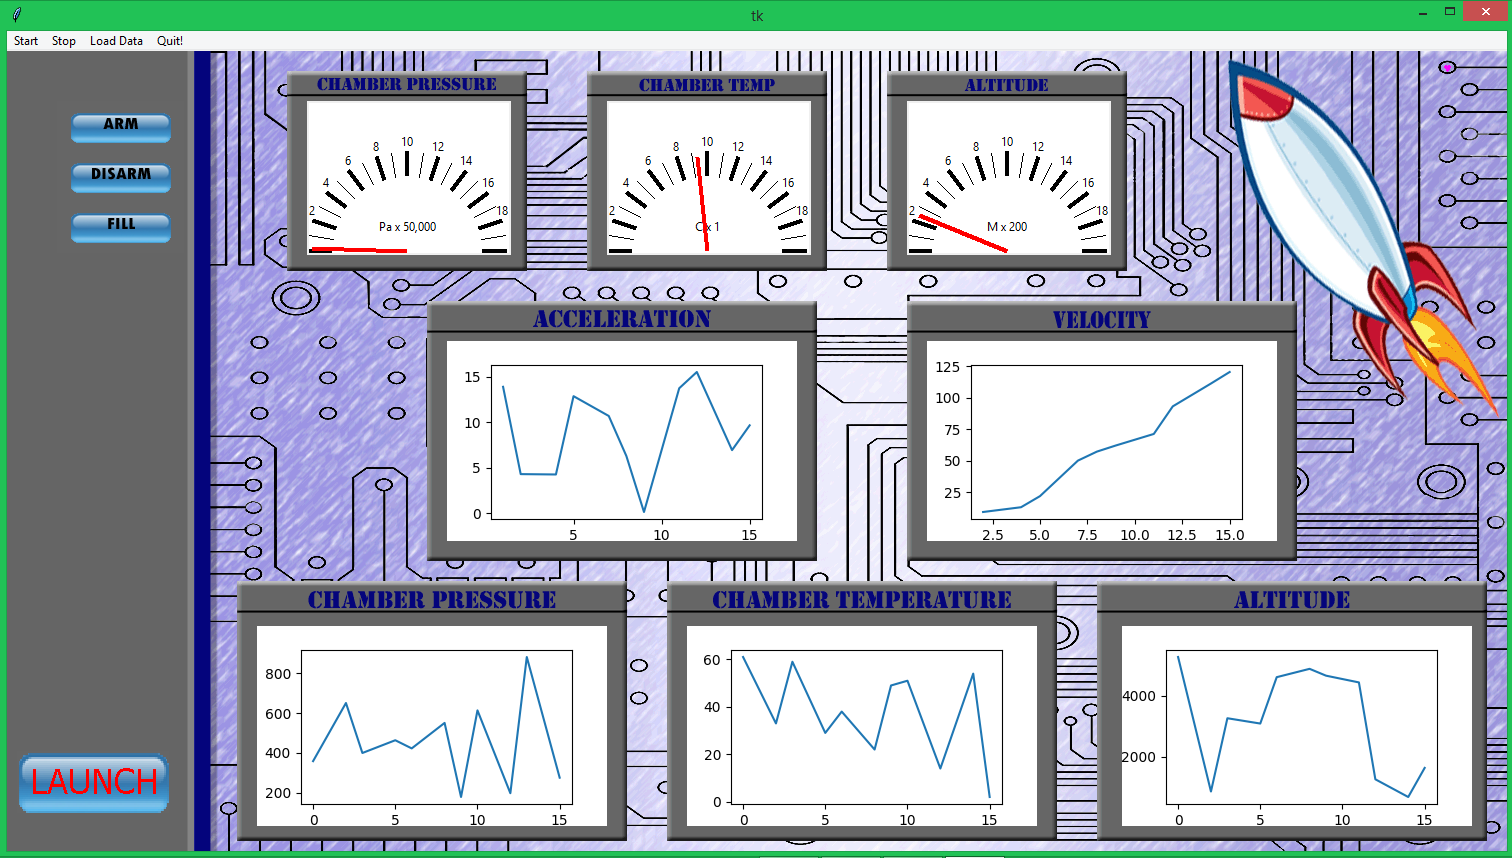
\includegraphics[scale=.45]{HyroGui}
\end{figure}

\subsection{The Command Buttons}
The command buttons are housed on the left side of the screen as depicted in the image above. These buttons will cause a command to be sent through the radio transceiver on the traditional computer to the radio transceiver on-board the rocket. The rocket will process the command and send a response back to be displayed in the message frame. The command buttons and their descriptions are as follows.\par

\begin{description}
\item[Fill] This will attempt to initiate the oxidizer fill process while the rocket is on the ground.
\end{description}

\subsection{The Main Menu}
A small menu will be provided at the top left hand side of the screen. It will bring up a file explorer window and allow you to chose what old data to load. This will initiate the data loading routines and the redraw functions. It also provides start and stop functions that will begin and end periods of radio communication. 

\subsection{The Gauges and Graphs}
Taking up most of the user interface on the right hand side are the gauges and graph canvases. Currently their will be 3 gauges that look like traditional gauges you would see on car dash board. They will be a semi circle with marks representing possible values of the data item. A arrow will be draw to represent the current value of the data. Below those gauges are 5 graphs representing all the different data items as graphs. Listed below are the gauges, graphs, and their units.

\subsubsection{Altitude Gauge}
{\bf Units} \\ Tick marks are measured in meters from 0 to 2000.\par
{\bf Description} \\ This gauge represents the current altitude of the rocket.\par

\subsubsection{Temperature Gauge}
{\bf Units} \\ Tick marks are measured in degrees Celsius from 0 to 500.\par
{\bf Description} \\ This gauge represents the temperature wherever the temperature sensor is located. It will rise and fall along with the temperature surrounding the temperature sensor.\par

\subsubsection{Chamber Pressure Gauge}
{\bf Units} \\ Tick marks are measured in pascals from 0 to 100.\par
{\bf Description} \\ This gauge represents the pressure of the avionics chamber of the rocket. It will rise and fall along with the chamber pressure of the rocket. \par

\subsubsection{Altitude Graph}
{\bf Units} \\ Time vs altitude graph. Altitude is displayed from 0 to 2000 meters.\par
{\bf Description} \\ This graph represents the altitude of the rocket. It will plot the altitude of the rocket vs time. \par

\subsubsection{Acceleration Graph}
{\bf Units} \\ The x axis of the graph will be measured in gs, the y axis will be time from launch in seconds.\par
{\bf Description} \\ This graph represents the acceleration of the rocket with respect to time. The graph will be able to slide if the amount of data points exceeds the size of the graph window. \par

\subsubsection{Velocity Graph}
{\bf Units} \\ The x axis of the graph will be measured in gs second and the y axis will be time from launch in seconds.\par
{\bf Description} \\ This graph represents the velocity of the rocket with respect to time. The graph will be able to slide if the amount of data points exceeds the size of the graph window. This graph is derived from acceleration data via numerical integration functions. \par

\subsubsection{Temperature Graph}
{\bf Units} \\ The x axis of the graph will be measured in Celsius and the y axis will be time from launch in seconds.\par
{\bf Description} \\ This graph represents temperature over time of the avionics bay in the rocket. The graph will be able to slide if the amount of data points exceeds the size of the graph window. \par

\subsubsection{Chamber Pressure Graph}
{\bf Units} \\ The x axis of the graph will be measured pascals and the y axis will be time from launch in seconds.\par
{\bf Description} \\ This graph represents the pressure over time of the rocket. The graph will be able to slide if the amount of data points exceeds the size of the graph window. \par


\section{Summary}
The previous section have in detailed described our hybrid rockets software system. We have described how we will collect sensors data, send sensor data, receive and act on commands, and provide  a command and visualization interface for the rocket team members on the ground. We have detailed the data formats, log formats, radio transceiver routines, data conversion routines, drawing routines and the threads that will control all these components. These are all housed in a threaded procedural system for simplicity and speed. All these components combined will allow for remote filling, launching, and data visualization of a hybrid rocket. \par

\newpage

\section{Bibliography}
\begin{thebibliography}{9}

\bibitem{BBB}
 BeagleBone.org,\\
\emph{(Tues November 29 2016)},\\
  \emph{Beagle Bone Black product information and website},\\
URL  http://beagleboard.org/black \\

\bibitem{ExampleSDD}
Unimap.edu example SDD,\\
\emph{(Tues November 29 2016)}, \\
  \emph{Unimap software development examples}, \\
URL http://portal.unimap.edu.my/portal/page/portal30/Lecturer\%20Notes/KEJURUTERAAN\_KOMPUTER/Semester\%202\%20Sidang\%20Akademik\%2020112012/EKT420\%20Software\%20Engineering/Example\%20of\%20Software\%20Design\%20Document(SDD)/EDDISS.pdf \\

\bibitem{IEE1016}
IEE 1016 Software Design Specifications,\\
\emph{(Tues November 29 2016)}, \\
  \emph{IEE 1016 Document availble on campus}, \\

\bibitem{TKinter}
Python.org wiki,\\
\emph{(Tues November 29 2016)}, \\
  \emph{Tkinter python wiki on python.org}, \\
URL https://wiki.python.org/moin/TkInter\\

\bibitem{Matplotlib}
Matplotlib.org,\\
\emph{(Tues November 29 2016)}, \\
  \emph{Matplotlib.org website documentation}, \\
URL http://matplotlib.org/

\end{thebibliography}

\newpage
\textbf{Students:}

\vspace{5mm}
 

\noindent \namesigdate{Jason Klindtworth} \hfill \namesigdate[6cm]{Josh Asher}
\vspace{5mm}

\noindent \namesigdate{Layne Nolli}
 \vspace{5mm}

\textbf{Client:}

\vspace{5mm}
 

\noindent \namesigdate{Nancy Squires}


\end{document}
